\item \textbf{{[}ALVL/9597/2017/P2/Q5{]} }The following grid shows the initial
state of a popular puzzle.
\begin{center}
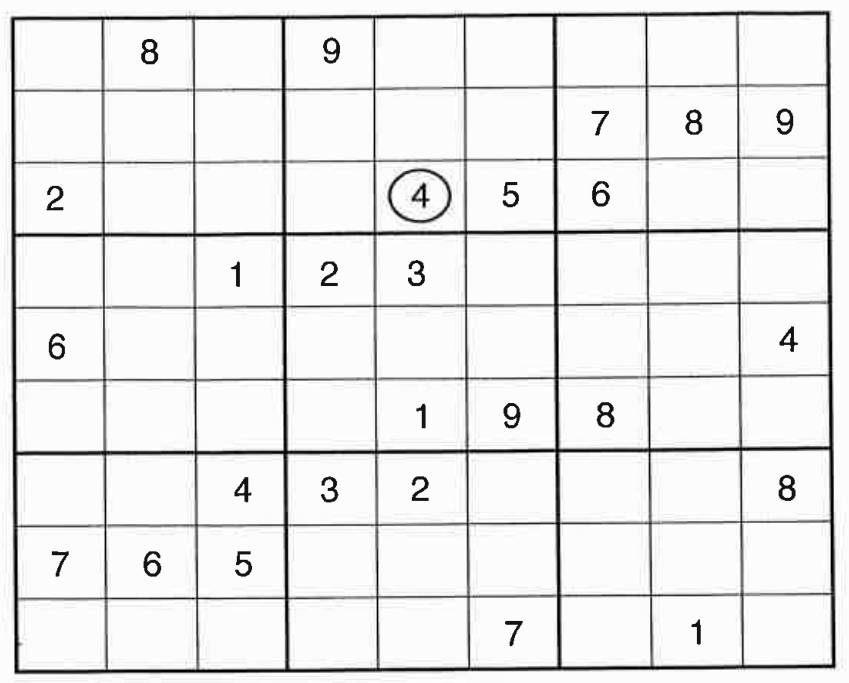
\includegraphics[width=0.5\paperwidth]{C:/Users/Admin/Desktop/Github/question_bank/LyX/static/img/9597-ALVL-2017-P2-Q5}
\par\end{center}

The aim of the puzzle is to fill the whole grid so that every row,
every column and every $3\times3$ mini-grid contains a number between
1 and 9. No number should be repeated in any row, column or 3 x 3
minigrid. 

A software company is creating an online version of the puzzle. A
programmer is asked to create the puzzle software. 
\begin{enumerate}
\item The programmer decides to use a 2D array to store the puzzle.
\begin{enumerate}
\item Copy and complete the following line of pseudocode. 

\texttt{DECLARE Puzzle ARRAY{[}1 : ...., .... : ....{]} OF ......................}
\hfill{}{[}2{]}

The circled value in the diagram above needs to be assigned to the
appropriate array element. 
\item Copy and complete the following line of pseudocode. 

\texttt{Puzzle{[}...., ....{]} <- ...............................}
\hfill{}{[}2{]}
\item Explain why a 2D array is more suitable than a single 1D array to
represent this puzzle. \hfill{}{[}2{]}
\end{enumerate}
\item The puzzle grid can be saved by writing the array \texttt{Puzzle}
to a file. 

Design an algorithm, using pseudocode, to write the array to the file.
\hfill{} {[}5{]}
\item During the testing of the puzzle software, several errors are discovered. 

Describe \textbf{two} debugging techniques that could be used to locate
these errors. \hfill{}{[}4{]}
\end{enumerate}